\chapter{Validation} \label{chap:validation}

\section*{}

To validate the framework 3 testbeds were prepared. The first is a collection 
of small fabricated test cases where we compare the output of multiple 
simulation runs to the expected results. The second and third cases deal with 
real uses of the framework, applied in two different e-commerce contexts: the 
first is an online store of computer products and the second is a general 
comparison shopping website.

% \section{Validation methodology}

\section{Sanity checks} % rename?

\subsection{Expected number of agents in the simulation}

This test compares the number of navigation agents expected to be 
\textit{alive} at each simulation step with the actual number of them.

At each simulation step, $k$ navigation agents enter the system and  
$p_{exit}$ of them leaves, which leads to the recurrence equation \ref{eq:recc}.

\begin{equation}\label{eq:recc}
\begin{cases}
a_{1} = \left (1 - p_{exit}  \right ) k\\
a_{n} = \left (1 - p_{exit}  \right ) \left (k + a_{n - 1} \right)
\end{cases} \Leftrightarrow a_{n} = \frac{k (p_{exit}-1) ((1-p_{exit})^{n} - 
1)}{p_{exit}}
\end{equation}

The simulation run was configured in the following way:

\begin{itemize}
    \item \textbf{Website}: Sample website with 9 pages and 32 total links 
    between pages
    \item \textbf{Website agent}: Dummy agent, does not modify any page;
    \item \textbf{Navigation agent}: Sample agent implementation with a chance 
    of exiting the website of $\frac{1}{3}$ ($p_{exit}$);
    \item \textbf{Number of new navigation agents each step}: 100 ($k$)
    \item \textbf{Number of simulation steps}: 1000
\end{itemize}

Replacing the values in equation \ref{eq:recc}: $a_{n} = -200 \left ( 
\frac{2}{3}^{n} - 1 \right )$. After a few simulation runs, the expected number 
of agents in the system stabilizes: $\lim_{n\to \infty} -200 \left ( 
\frac{2}{3}^{n} - 1 \right ) = 200$.

The results of a simulation run were gathered and plotted in figure 
\ref{fig:expagents}. Triangles ($\triangle$) represent the actual value 
($A_{t}$) and circles ($\bullet$) represent the expected value ($E_{t}$) 
according to the equations above. SMAPE (symmetric mean absolute percentage 
error)\cite{makridakis1993accuracy} is used to measure the accuracy of the 
results: $ SMAPE = {\frac {1}{n}}\sum _{t=1}^{n}{\frac 
{\left|E_{t}-A_{t}\right|}{|A_{t}|+|E_{t}|}} = 3.07\% $, which is a reasonable 
low \textit{error} rate given the randomness of the system.

\begin{figure}[h]
    \begin{center}
        \leavevmode
        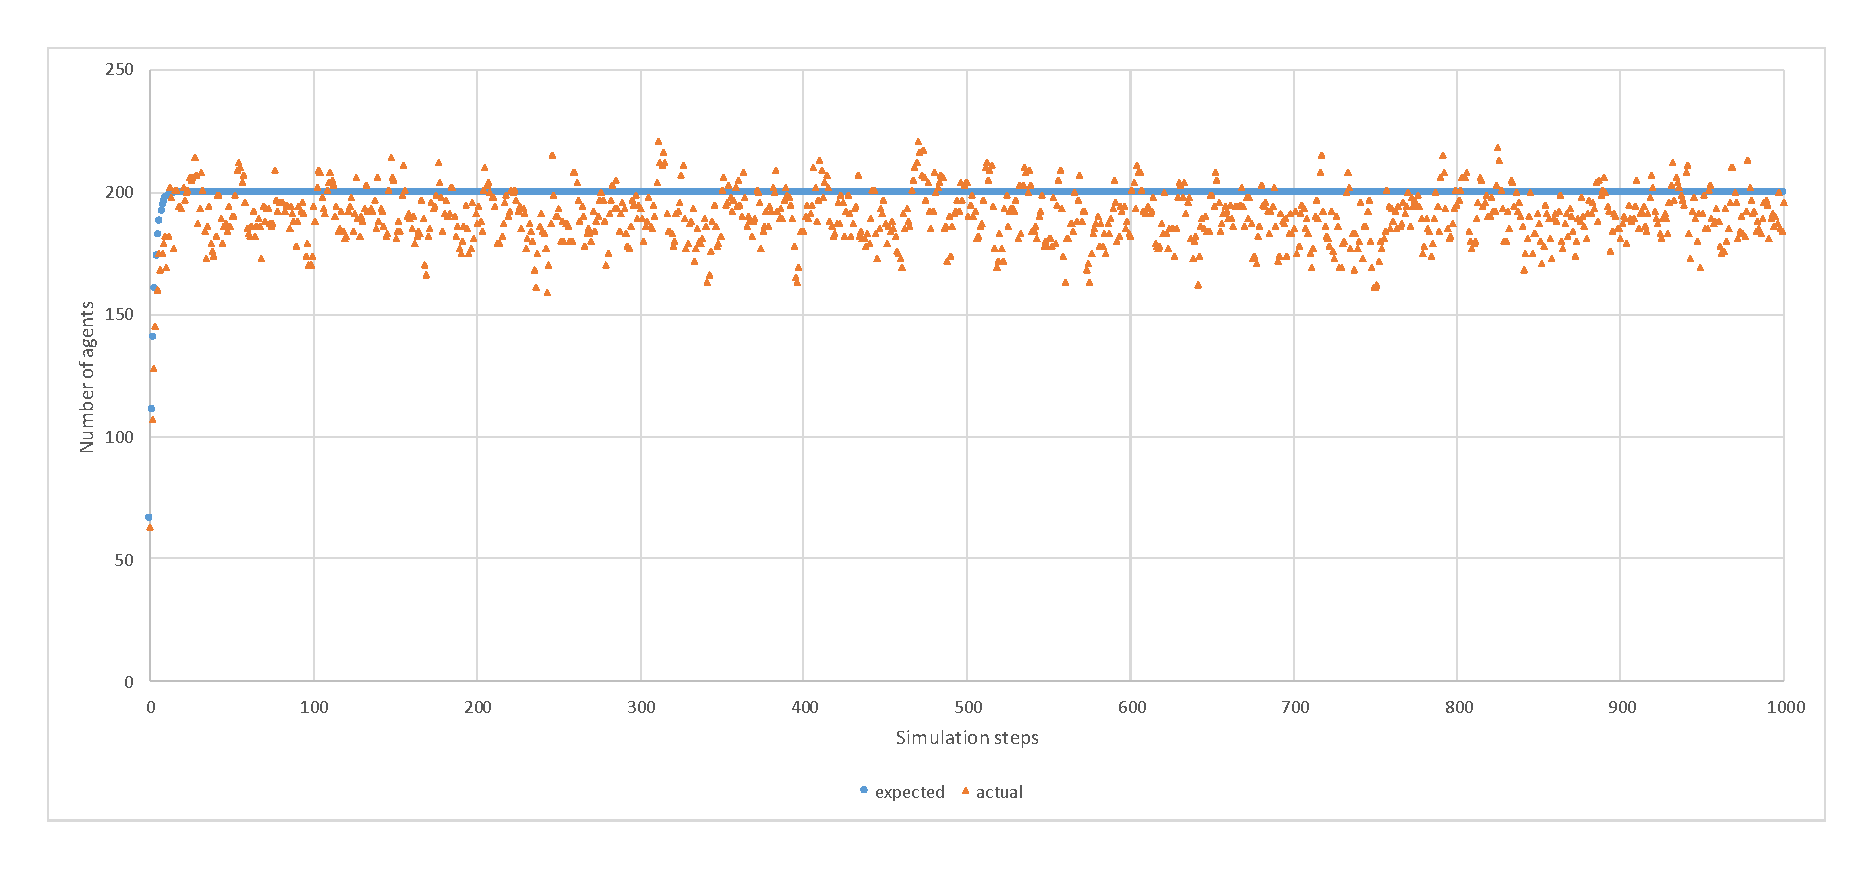
\includegraphics[width=0.95\textwidth]{expected_agents}
        \caption{Expected number of agents in the simulation}
        \label{fig:expagents}
    \end{center}
\end{figure}

\subsection{Expected number of visits}

This test compares the number of visits (page hits) for a given website and 
agents setup. The simulation run was configured in the following way:

\begin{itemize}
    \item \textbf{Website}: Website configured as displayed in figure 
    \ref{fig:test2website}. The homepage links to 5 product pages and the 
    product page link to the cart page.
    \item \textbf{Website agent}: Dummy agent, does not modify any page;
    \item \textbf{Navigation agent}: The agent picks one linked page randomly 
    however if current page is for a product, it always buys it. If the current 
    page is the cart page, it leaves the website;
    \item \textbf{Number of new navigation agents each step}: 100
    \item \textbf{Number of simulation steps}: 1000
\end{itemize}

\begin{figure}
\centering
\begin{tikzpicture}
\SetGraphUnit{3}
\GraphInit[vstyle=Welsh]
\tikzset{VertexStyle/.append style = { minimum size = 24pt}}
\Vertex{page3}
\WE(page3){page2}
\WE(page2){page1}
\EA(page3){page4}
\EA(page4){page5}
\NO(page3){homepage}
\SO(page3){cart}
\tikzset{EdgeStyle/.append style = {->}}
\Edge(homepage)(page1)
\Edge(homepage)(page2)
\Edge(homepage)(page3)
\Edge(homepage)(page4)
\Edge(homepage)(page5)
\tikzset{EdgeStyle/.append style = {->}}
\Edge(page1)(cart)
\Edge(page2)(cart)
\Edge(page3)(cart)
\Edge(page4)(cart)
\Edge(page5)(cart)
% \tikzset{EdgeStyle/.append style = {->,bend left}}
% \Edge(cart)(homepage)
\end{tikzpicture}
\caption{Website graph for the expected visits test} \label{fig:test2website}
\end{figure}

The table \ref{tab:test2results} displays the expected and observed number of 
visits for a simulation run as described above. The percent error is calculated 
and the obtained results are very close to the predicted values.

\begin{table}[]
    \centering
    \caption{Expected and observed number of visits}
    \label{tab:test2results}
    \begin{tabular}{@{}lllll@{}}
        \toprule
        Page     & Observed   & \multicolumn{2}{l}{Expected} & Error  \\ 
        \midrule
        homepage & $100000$   & $100 \times 1000$ & $ = 100000$      & $0.00\%$ 
        \\
        page1    & $19864$    & $\frac{1}{5} \times 100 \times 1000$ & $ = 
        20000$ &         $0.68\%$ \\
        page2    & $20100$    & $\frac{1}{5} \times 100 \times 1000$ & $ = 
        20000$ &         $0.50\%$ \\
        page3    & $19696$    & $\frac{1}{5} \times 100 \times 1000$ & $ = 
        20000$ &         $1.52\%$ \\
        page4    & $20096$    & $\frac{1}{5} \times 100 \times 1000$ & $ = 
        20000$ &         $0.48\%$ \\
        page5    & $20244$    & $\frac{1}{5} \times 100 \times 1000$ & $ = 
        20000$ &         $1.22\%$ \\
        cart     & $99900$    & $20000 \times 5$ & $ = 100000$       & $0.10\%$ 
        \\ 
        \bottomrule
    \end{tabular}
\end{table}

\subsection{Expected bounce rate}

This case compares the bounce rate for a website that only has one page. We 
define the bounce rate as the percentage of navigation agent sessions that only 
view a single page before existing the website.

The simulation run was configured in the following way:

\begin{itemize}
    \item \textbf{Website}: One page only, the homepage;
    \item \textbf{Website agent}: Dummy agent, does not modify any page;
    \item \textbf{Navigation agent}: Agent that picks its actions randomly;
    \item \textbf{Number of new navigation agents each step}: 100
    \item \textbf{Number of simulation steps}: 1000
\end{itemize}

As expected, the simulation results yield $100\%$ bounce rate, all of the 
visits were to the homepage, $10000$ unique users ($100 \times 1000$) and no 
purchases, as it can be seen on figure \ref{fig:test3result}.

\begin{figure}[h]
    \begin{center}
        \leavevmode
        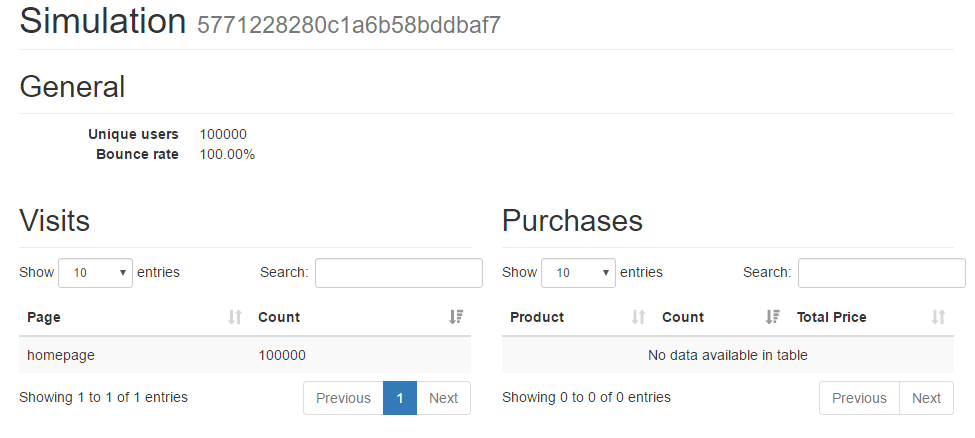
\includegraphics[width=0.95\textwidth]{expected_bounce_rate}
        \caption{Screenshot of the frontend results for this test run}
        \label{fig:test3result}
    \end{center}
\end{figure}

% \subsection{ test conversion rate, always buy -> 100% }

\section{Online store}

\subsection{Input data and configuration}
\subsection{Simulation}
\subsection{Results}

\section{Comparison shopping website}

\subsection{Input data and configuration}
\subsection{Simulation}
\subsection{Results}
